% Completa los datos convenientemente en las zonas marcadas con TODO

\documentclass{beamer}
%PARA VISUALIZAR PRESENTACIONN CON NOTAS USAR VISUALIZADOR "pdfpc":
%Para ver las notas, el cronometro y siguente diapo:
% pdfpc --notes=right slides.pdf
% "tecla p": para pausar el cronometro
\mode<presentation> {
  \usetheme{CambridgeUS}
  \usecolortheme{crane} % color naranja
}
\setbeamercolor{titlelike}{parent=structure,bg=yellow!85!orange} % Cambia el color de la caja del título de la página inicial

\setbeamertemplate{navigation symbols}{} % ocultar iconos de navegación
\setbeamerfont{subsection in toc}{size=\small} % reducir tamaño en TOC
\setbeamerfont{date}{size=\tiny}
\usepackage[spanish]{babel}
\usepackage[utf8]{inputenc}
\usepackage{graphicx}
\usepackage{eurosym}
\usepackage{booktabs}
\usepackage{hyperref}
\usepackage{graphicx}
\usepackage{multicol}
\usepackage{pgfpages}
\usepackage{listings}
\usepackage{multimedia}
\usepackage[export]{adjustbox}
\usepackage{outlines} % Para poner bullets tabulados (\1 \2 \3 ...) y no items

\usepackage{array,tabularx} % para tabular leyenda de ecuaciones
\newenvironment{conditions*} % entorno de "leyenda de ecuación"
  {\par\vspace{\abovedisplayskip}\noindent
   \tabularx{\columnwidth}{>{$}l<{$} @{\ : } >{\raggedright\arraybackslash}X}}
  {\endtabularx\par\vspace{\belowdisplayskip}}
  
% USO DE NOTAS
\setbeameroption{hide notes} % Para mostrar u ocultar (hide/show)
%\setbeameroption{show only notes} % Mostrar solo las notas
%\setbeameroption{show notes on second screen=right} % Mostrar notas en otra pantalla
\setbeamertemplate{note page}{ % asi solo muestro el texto de las notas
  \insertnote%
}

%========= TODO: datos internos del documento
\hypersetup{
	pdftitle={Defensa de trabajo de fin de grado de Vidal Pérez Bohoyo},
	pdfauthor={Vidal Pérez Bohoyo},
	pdfsubject={Brazo robótico de bajo coste para la docencia universitaria},
	pdfkeywords={teaching, robotics, arm, ROS, actuators, DOF, 3D, printer},
	pdfproducer={pdfLaTeX},
  colorlinks=true,
  linkcolor=blue
}
%=========

%========= TODO: diapositiva de portada
\title[Brazo robótico de bajo coste]{Brazo robótico de bajo coste para la docencia universitaria} % El título reducido aparece en la parte inferior de todas las diapositivas
                                         % El título completo aparece solo en la diapositiva de portada
\author[Vidal Pérez Bohoyo]{Vidal Pérez Bohoyo}
\institute[URJC]
{
\textit{\href{mailto:v.perezb.2019@alumnos.urjc.es}{\color{blue}{\underline{v.perezb.2019@alumnos.urjc.es}}}}\\
\vspace{0.5cm}

\includegraphics[width=3cm]{figs/logo-urjc}\\
\vspace{1cm}
Trabajo fin de grado
}
\date{xx de xxxxxxx de 20xx}
%=========

%========= COMIENZO DEL DOCUMENTO
\begin{document}

%========= Portada inicial con notas
\begin{frame}[plain] % plain: quita header y footer
\large{\titlepage}
\note[item]{En esta presentación voy a hablar sobre...}
\note[item]{En primer lugar...}
\end{frame}

%========= Licencia
\begin{frame}
% Este diseño se corresponde con la licencia CC-BY-NC-SA.
% Por supuesto, puedes poner la licencia que mejor se adapte al propósito de tu trabajo.
% Recuerda que, si no se especifica ninguna licencia, esta -como cualquier creación artística- pasaría a estar licenciada con todos los derechos reservados (copyright).

\cleardoublepage

\begin{figure}
 \ \ \ \ 
\includegraphics[width=0.25\linewidth]{figs/by-nc-sa.png}
 \label{fig:cc} 
 \end{figure}

\

\

\

\noindent
Este trabajo se distribuye bajo los términos de la licencia internacional \href{http://creativecommons.org/licenses/by-nc-sa/4.0/}{CC BY-NC-SA International License} (Creative Commons AttributionNonCommercial-ShareAlike 4.0). Usted es libre de \textit{(a) compartir}: copiar y redistribuir el material en cualquier medio o formato; y \textit{(b) adaptar}: remezclar, transformar y crear a partir del material. El licenciador no puede revocar estas libertades mientras cumpla con los términos de la licencia:

\begin{itemize}
\item \textit{Atribución}. Usted debe dar crédito de manera adecuada, brindar un enlace a la licencia, e indicar si se han realizado cambios. Puede hacerlo en cualquier forma razonable, pero no de forma tal que sugiera que usted o su uso tienen el apoyo de la licenciante.
\item \textit{No comercial}. Usted no puede hacer uso del material con propósitos comerciales.
\item \textit{Compartir igual}. Si remezcla, transforma o crea a partir del material, debe distribuir su contribución bajo la la misma licencia del original.
\end{itemize}

\begin{flushright}
		\vspace{7.0 cm}
		\emph{Documento de} \textbf{Vidal Pérez Bohoyo}. 
\end{flushright}


\end{frame}

%========= Índice o tabla de contenidos (TOC)
\begin{frame}
\frametitle{Contenidos}
%\begin{multicols}{2} % si tengo muchas secciones, lo parte en dos columnas
  \tableofcontents[hideallsubsections] % no muestra subsecciones
%\end{multicols}
\note[item]{La presentaci\'on esta dividida en cuatro partes.}
\end{frame}

%========= Diapositiva "vacía" de comienzo de sección:
\section*{}
\begin{frame}{}
  \centering \Huge
  \emph{Introducción}
\note[item]{Comencemos con la introducción.}
\end{frame}

\section{Introducción}
\subsection{Contexto general}


\begin{frame}
\frametitle{Robótica industrial}

\end{frame}

\begin{frame}
\frametitle{Robótica educativa}

\end{frame}

\begin{frame}
\frametitle{Robótica de bajo coste}

\end{frame}

%========= Diapositiva con ítems resaltados con colores:
\begin{frame}
\frametitle{Situación de la Robótica}
\begin{itemize}
\item La \textcolor{red}{tecnología} está cada vez más presente en la vida cotidiana.
\item Los robots de servicio aparecen en el \textcolor{blue}{mercado}.
\item La \textcolor{red}{domótica} presenta cada vez más aplicaciones domésticas.
\end{itemize}
\end{frame}

\subsection{Contexto específico}
%========= Diapositiva con bloques:
\begin{frame}
\frametitle{Precedentes de la robótica}
\begin{block}{Primera revolución industrial de 1800}
Productos fabricados por \textcolor{blue}{máquinas}. La \textcolor{red}{máquina de vapor} fue clave.
\end{block}
\end{frame}

\section*{}
\begin{frame}{}
  \centering \Huge
  \emph{Objetivos}
\note[item]{Pasemos ahora a comentar los objetivos que nos hemos con este trabajo.}
\end{frame}

\begin{frame}
\frametitle{Descripción del problema}
\begin{block}{Primera revolución industrial de 1800}
Productos fabricados por \textcolor{blue}{máquinas}. La \textcolor{red}{máquina de vapor} fue clave.
\end{block}
\end{frame}
  
\begin{frame}
\frametitle{Requisitos}
\begin{enumerate}
\item Coste inferior a 200\euro.
\item En su mayoría impreso en 3D.
\item Bajo consumo eléctrico, inferior a 25 vatios.
\item Tamaño reducido.
\item Sencillo de montar.
\item Tener integración con ROS 2 y MoveIt 2.
\end{enumerate}
\end{frame}

\begin{frame}
\frametitle{Metodología}

\end{frame}

\section*{}
\begin{frame}{}
  \centering \Huge
  \emph{Plataforma de desarrollo}
\note[item]{Una vez descritos los objetivos, veamos qué hemos hecho para alcanzarlos.}
\end{frame}

\begin{frame}
\frametitle{Software}
\begin{table}[htbp]
  \centering
  \begin{tabular}{ccc}
      
\includegraphics[width=0.3\textwidth, valign=m]{figs/phyton.jpg} & 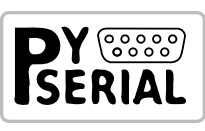
\includegraphics[width=0.2\textwidth, valign=m]{figs/pyserial.png} &
      
\includegraphics[width=0.2\textwidth, valign=m]{figs/grbl.png} \\
      
\includegraphics[width=0.3\textwidth, valign=m]{figs/freecad.png} & 
\includegraphics[width=0.2\textwidth, valign=m]{figs/ros2logo.jpeg} & 
      
\includegraphics[width=0.3\textwidth, valign=m]{figs/moveit2.png}
  \end{tabular}
\end{table}
\end{frame}

\begin{frame}
\frametitle{Hardware}
\begin{table}[htbp]
  \centering
  \begin{tabular}{ccc}
      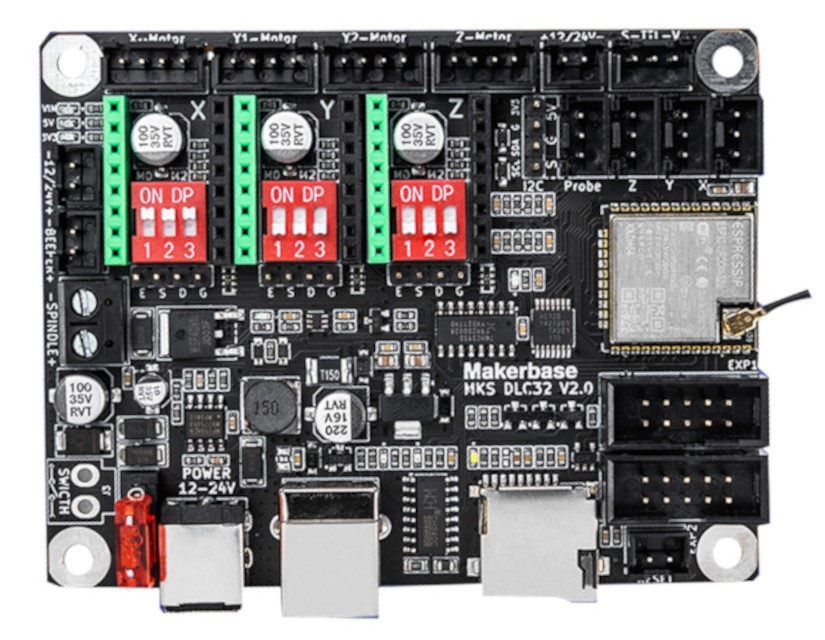
\includegraphics[width=0.2\textwidth, valign=m]{figs/mksdlc32.jpg} & 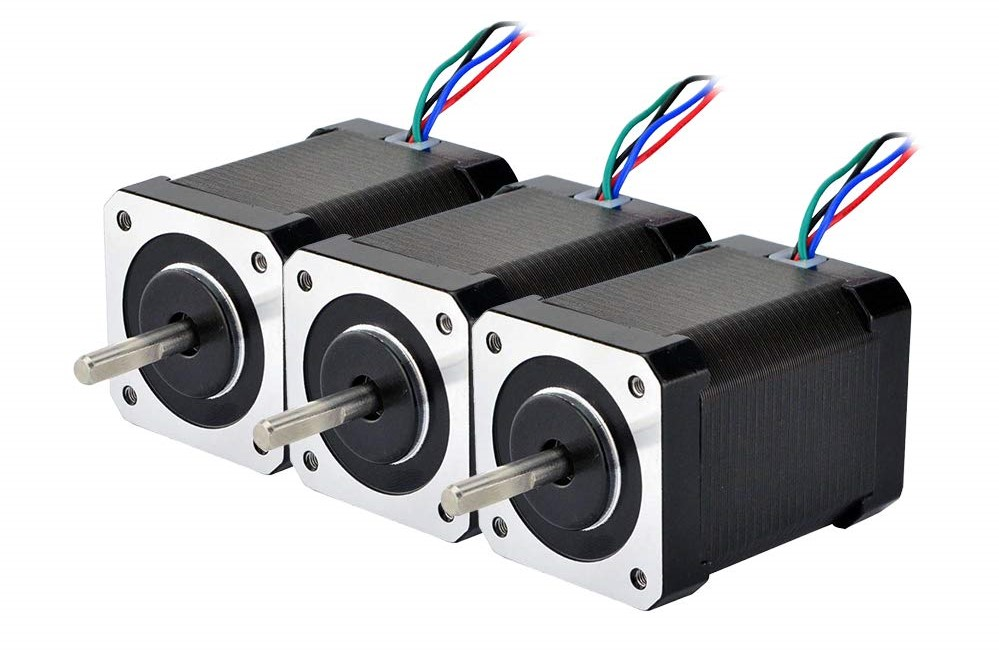
\includegraphics[width=0.2\textwidth, valign=m]{figs/nema17.jpg} &
      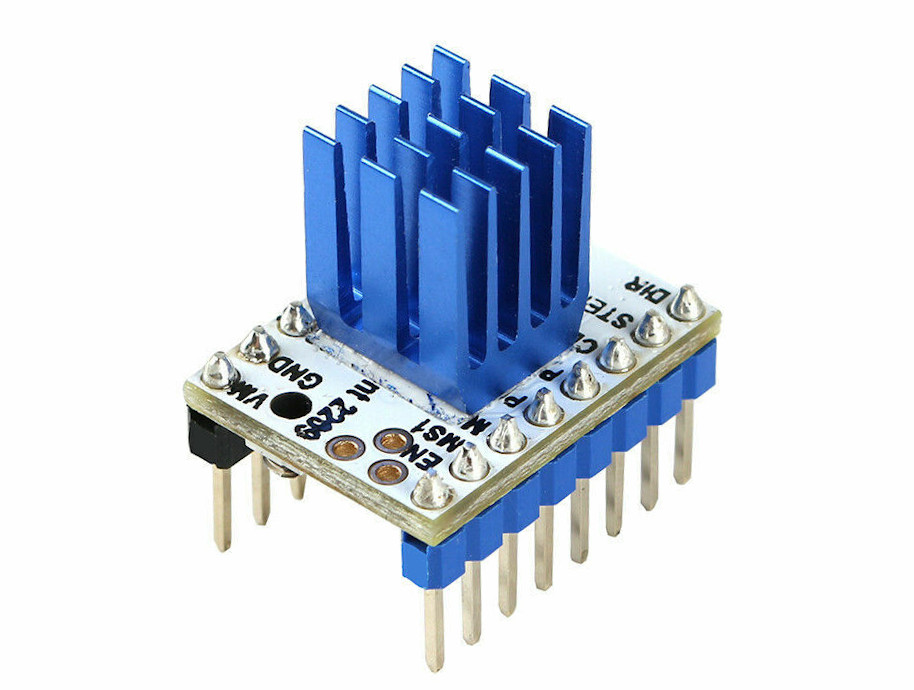
\includegraphics[width=0.2\textwidth, valign=m]{figs/TMC2209.jpg} \\
      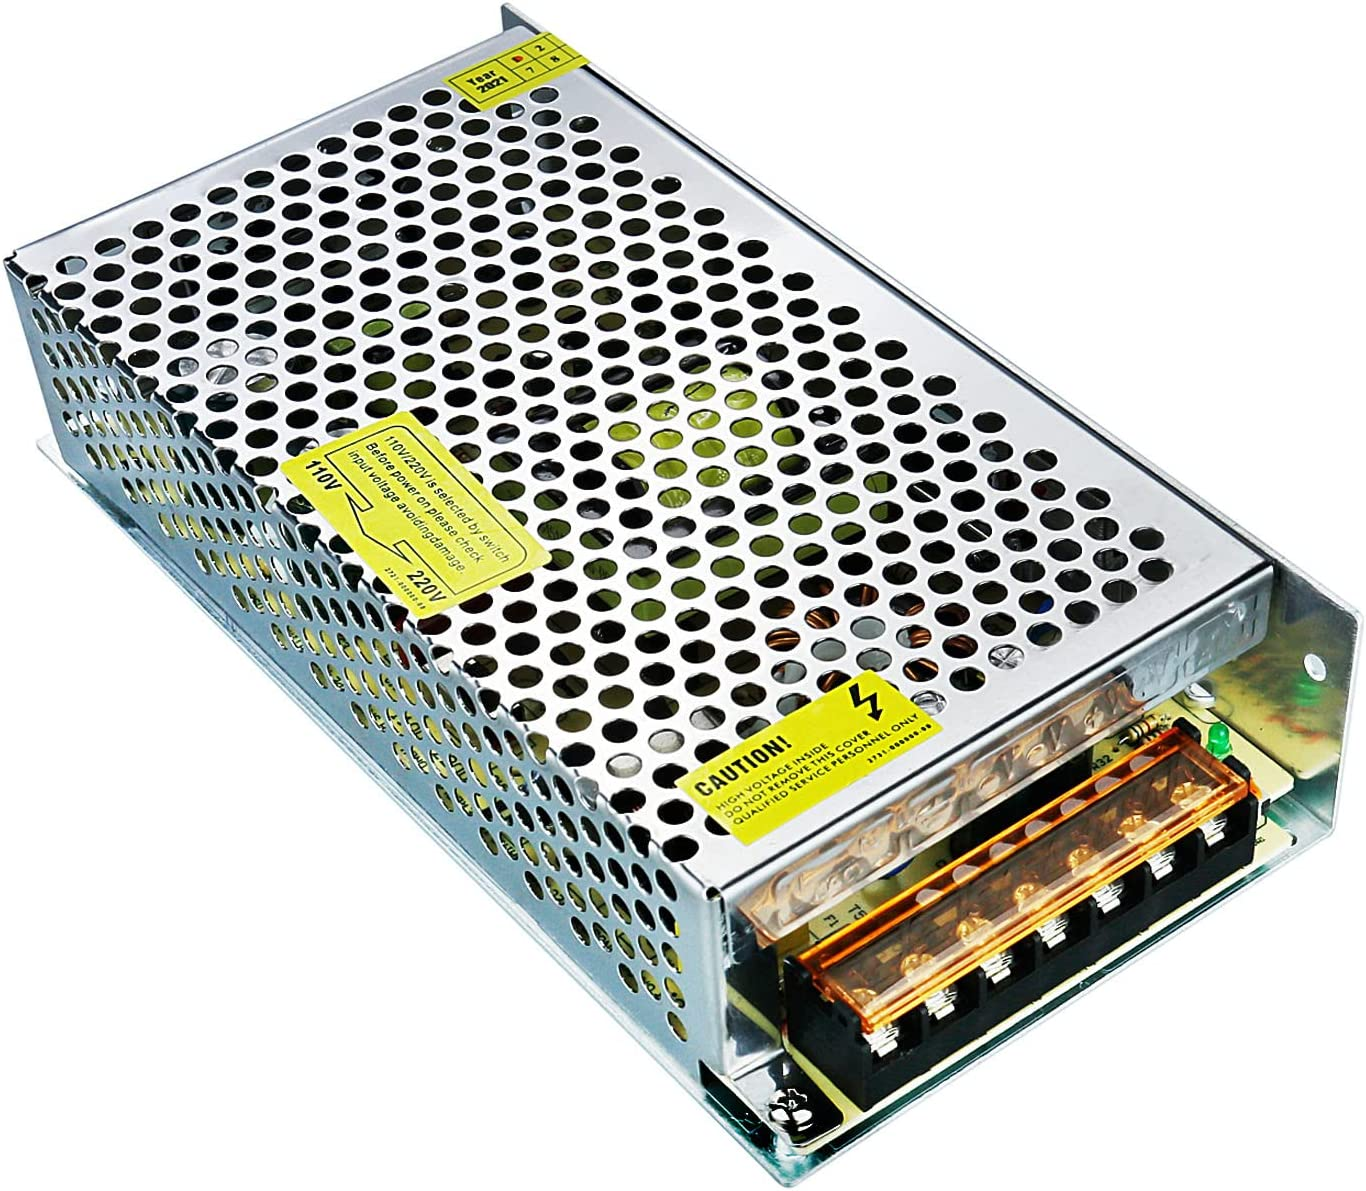
\includegraphics[width=0.2\textwidth, valign=m]{figs/pw24v.jpg} & 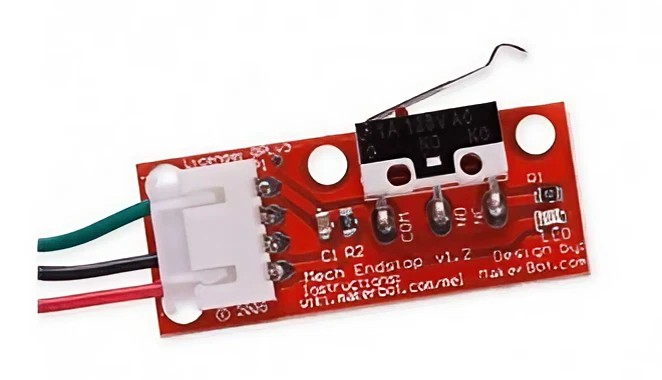
\includegraphics[width=0.2\textwidth, valign=m]{figs/finaldecarrera.jpg} & 
      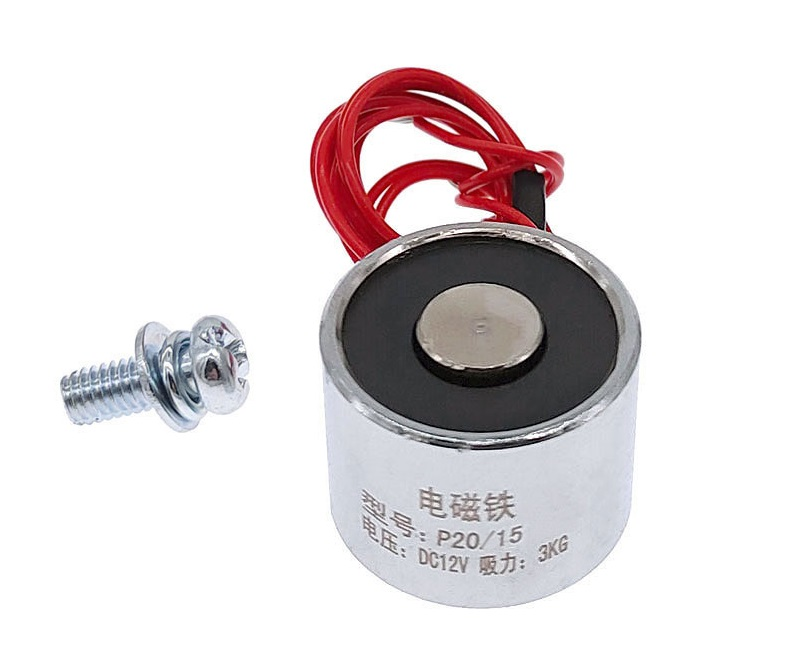
\includegraphics[width=0.2\textwidth, valign=m]{figs/d20h15.jpg} \\ 
      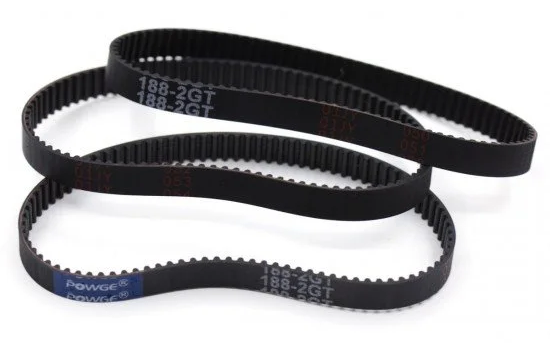
\includegraphics[width=0.2\textwidth, valign=m]{figs/correa.png} & 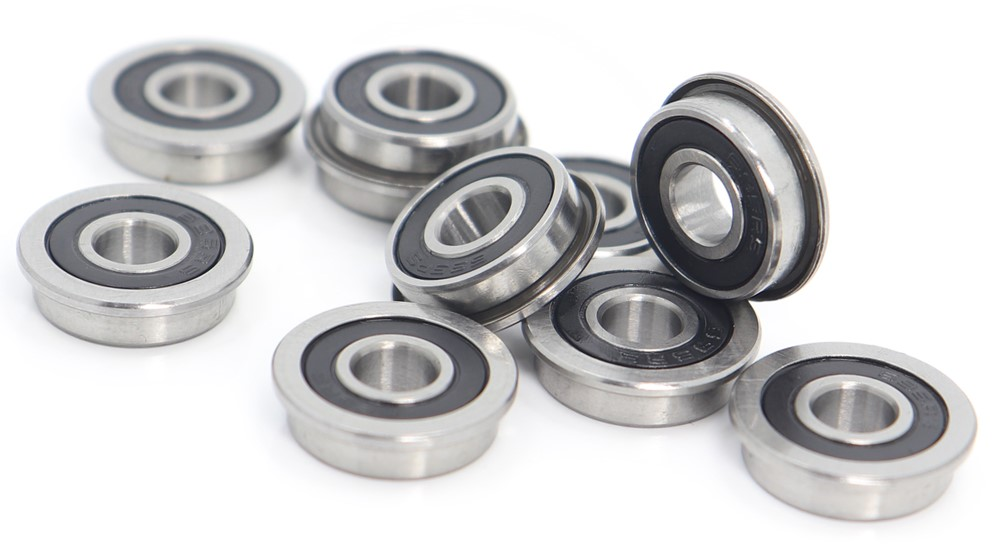
\includegraphics[width=0.2\textwidth, valign=m]{figs/F695-2RS.jpeg} & 
      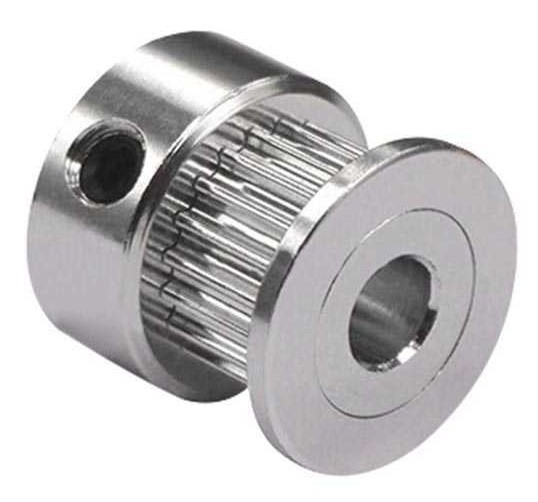
\includegraphics[width=0.12\textwidth, valign=m]{figs/20t.jpg}
  \end{tabular}
\end{table}
\end{frame}

\begin{frame}
\end{frame}

\section*{}
\begin{frame}{}
  \centering \Huge
  \emph{Desarrollo hardware}
\note[item]{Una vez descritos los objetivos, veamos qué hemos hecho para alcanzarlos.}
\end{frame}

\section*{}
\begin{frame}{}
  \centering \Huge
  \emph{Desarrollo software}
\note[item]{Una vez descritos los objetivos, veamos qué hemos hecho para alcanzarlos.}
\end{frame}

\begin{frame}
\frametitle{Grbl y comunicación con el ordenador}
\begin{figure}[h]
  \centering
  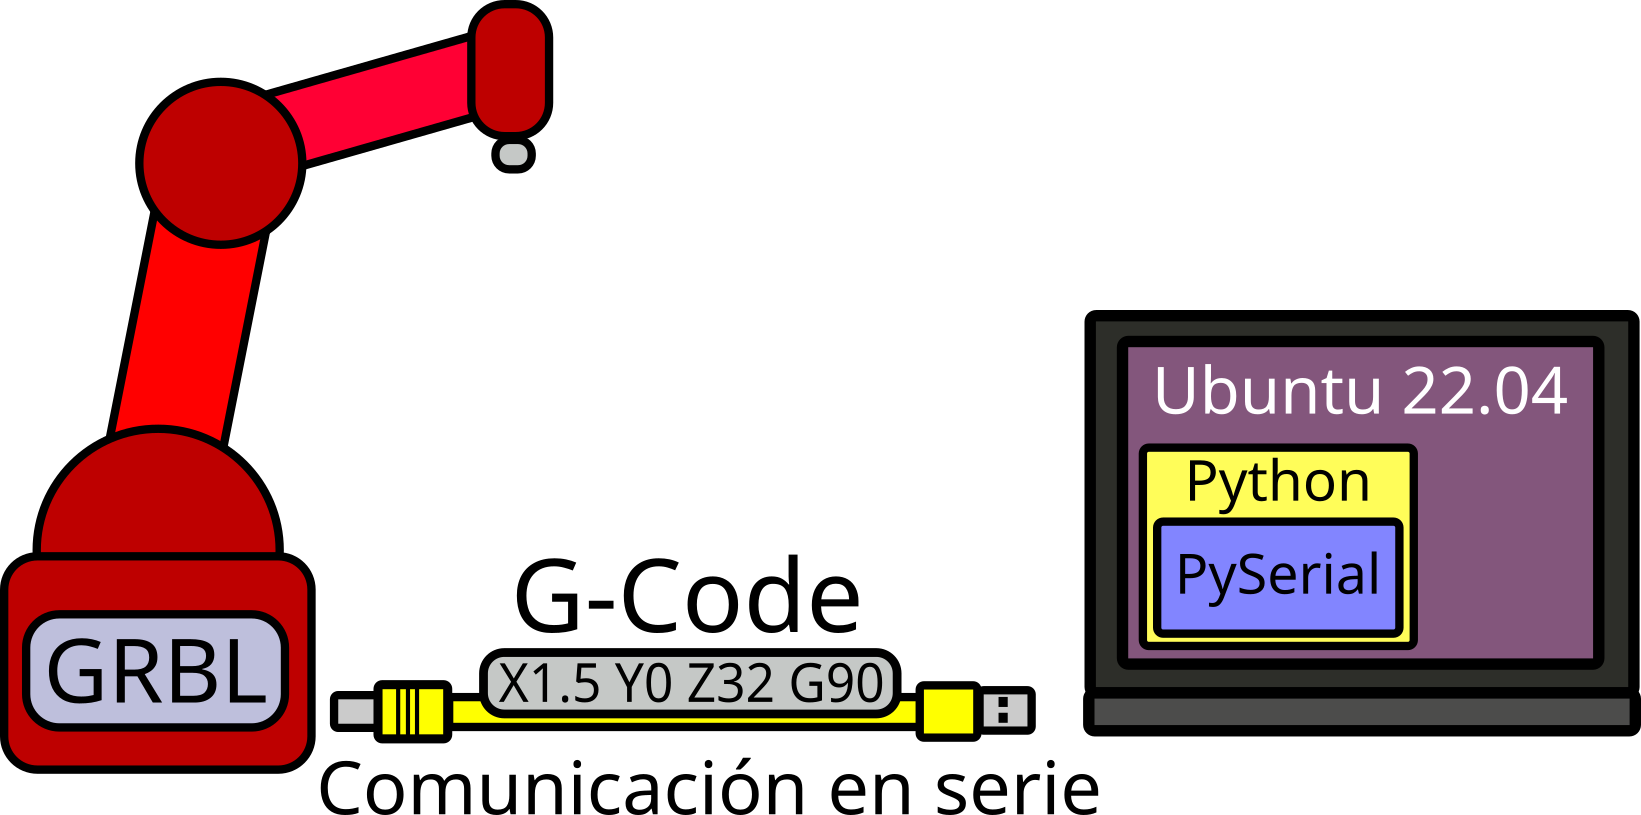
\includegraphics[width=0.8\textwidth]{figs/coms.png}
\end{figure}
\end{frame}

\begin{frame}
\frametitle{Integración con ROS 2}
\begin{table}[htbp]
  \centering
  \begin{tabular}{ccc}
      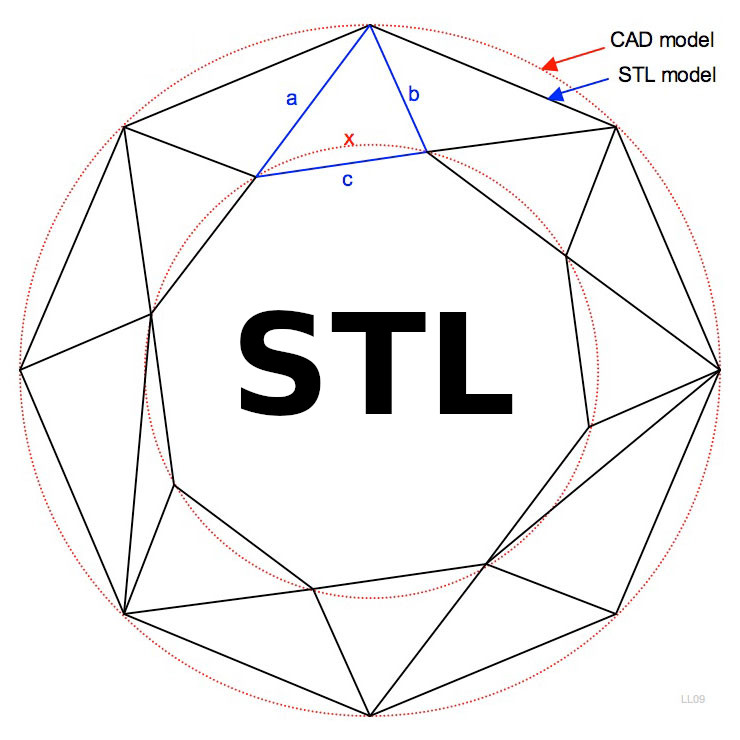
\includegraphics[width=0.15\textwidth, valign=m]{figs/STL.jpg} & 
\includegraphics[width=0.3\textwidth, valign=m]{figs/collada.png} 
       & 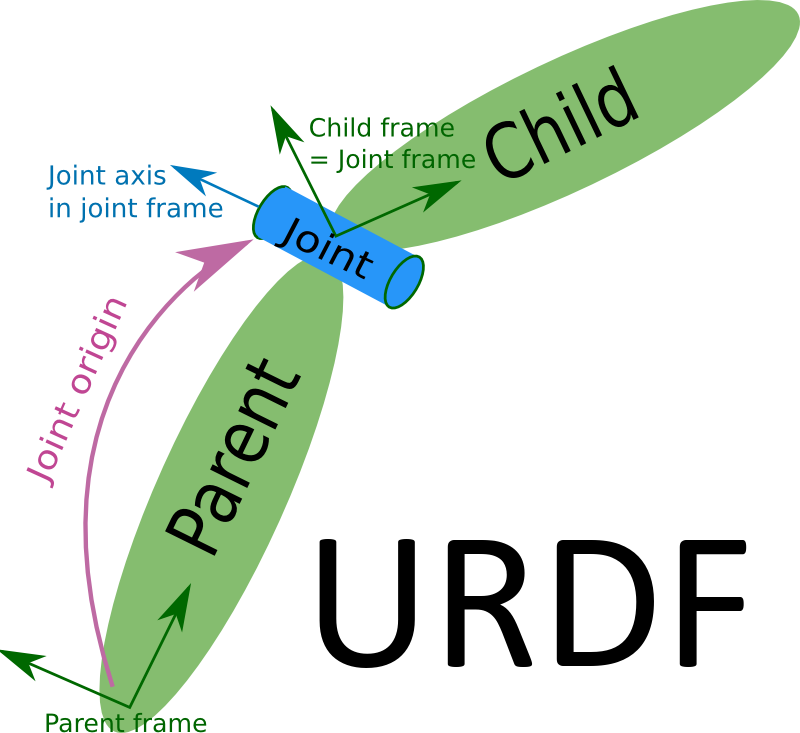
\includegraphics[width=0.15\textwidth, valign=m]{figs/urdf.png} \\
      
  \end{tabular}
\end{table} 
\begin{figure}[h]
  
\centering
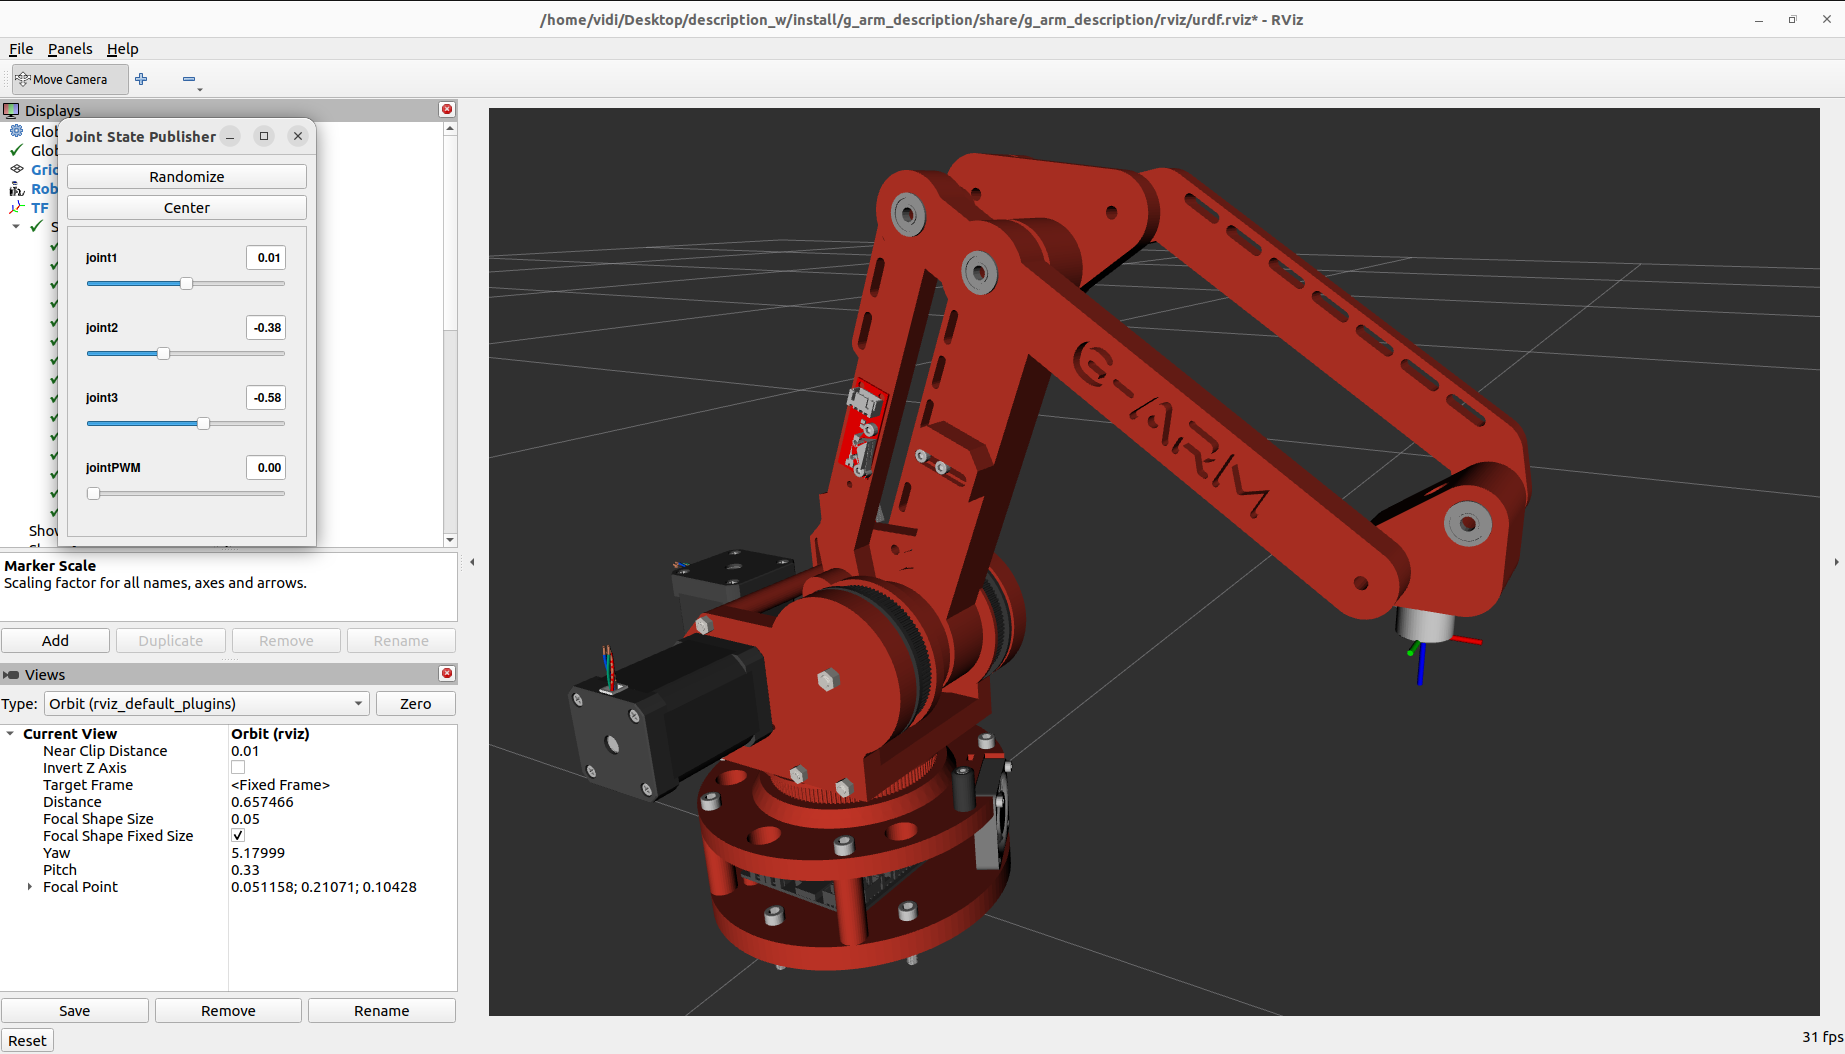
\includegraphics[width=0.7\textwidth]{figs/rviz.png}
\end{figure}  
\end{frame}

\begin{frame}
\frametitle{Integración con MoveIt 2}
\begin{table}[htbp]
  \centering
  \begin{tabular}{cc}
      
\includegraphics[width=0.2\textwidth, valign=m]{figs/setup_assistant.jpg} & 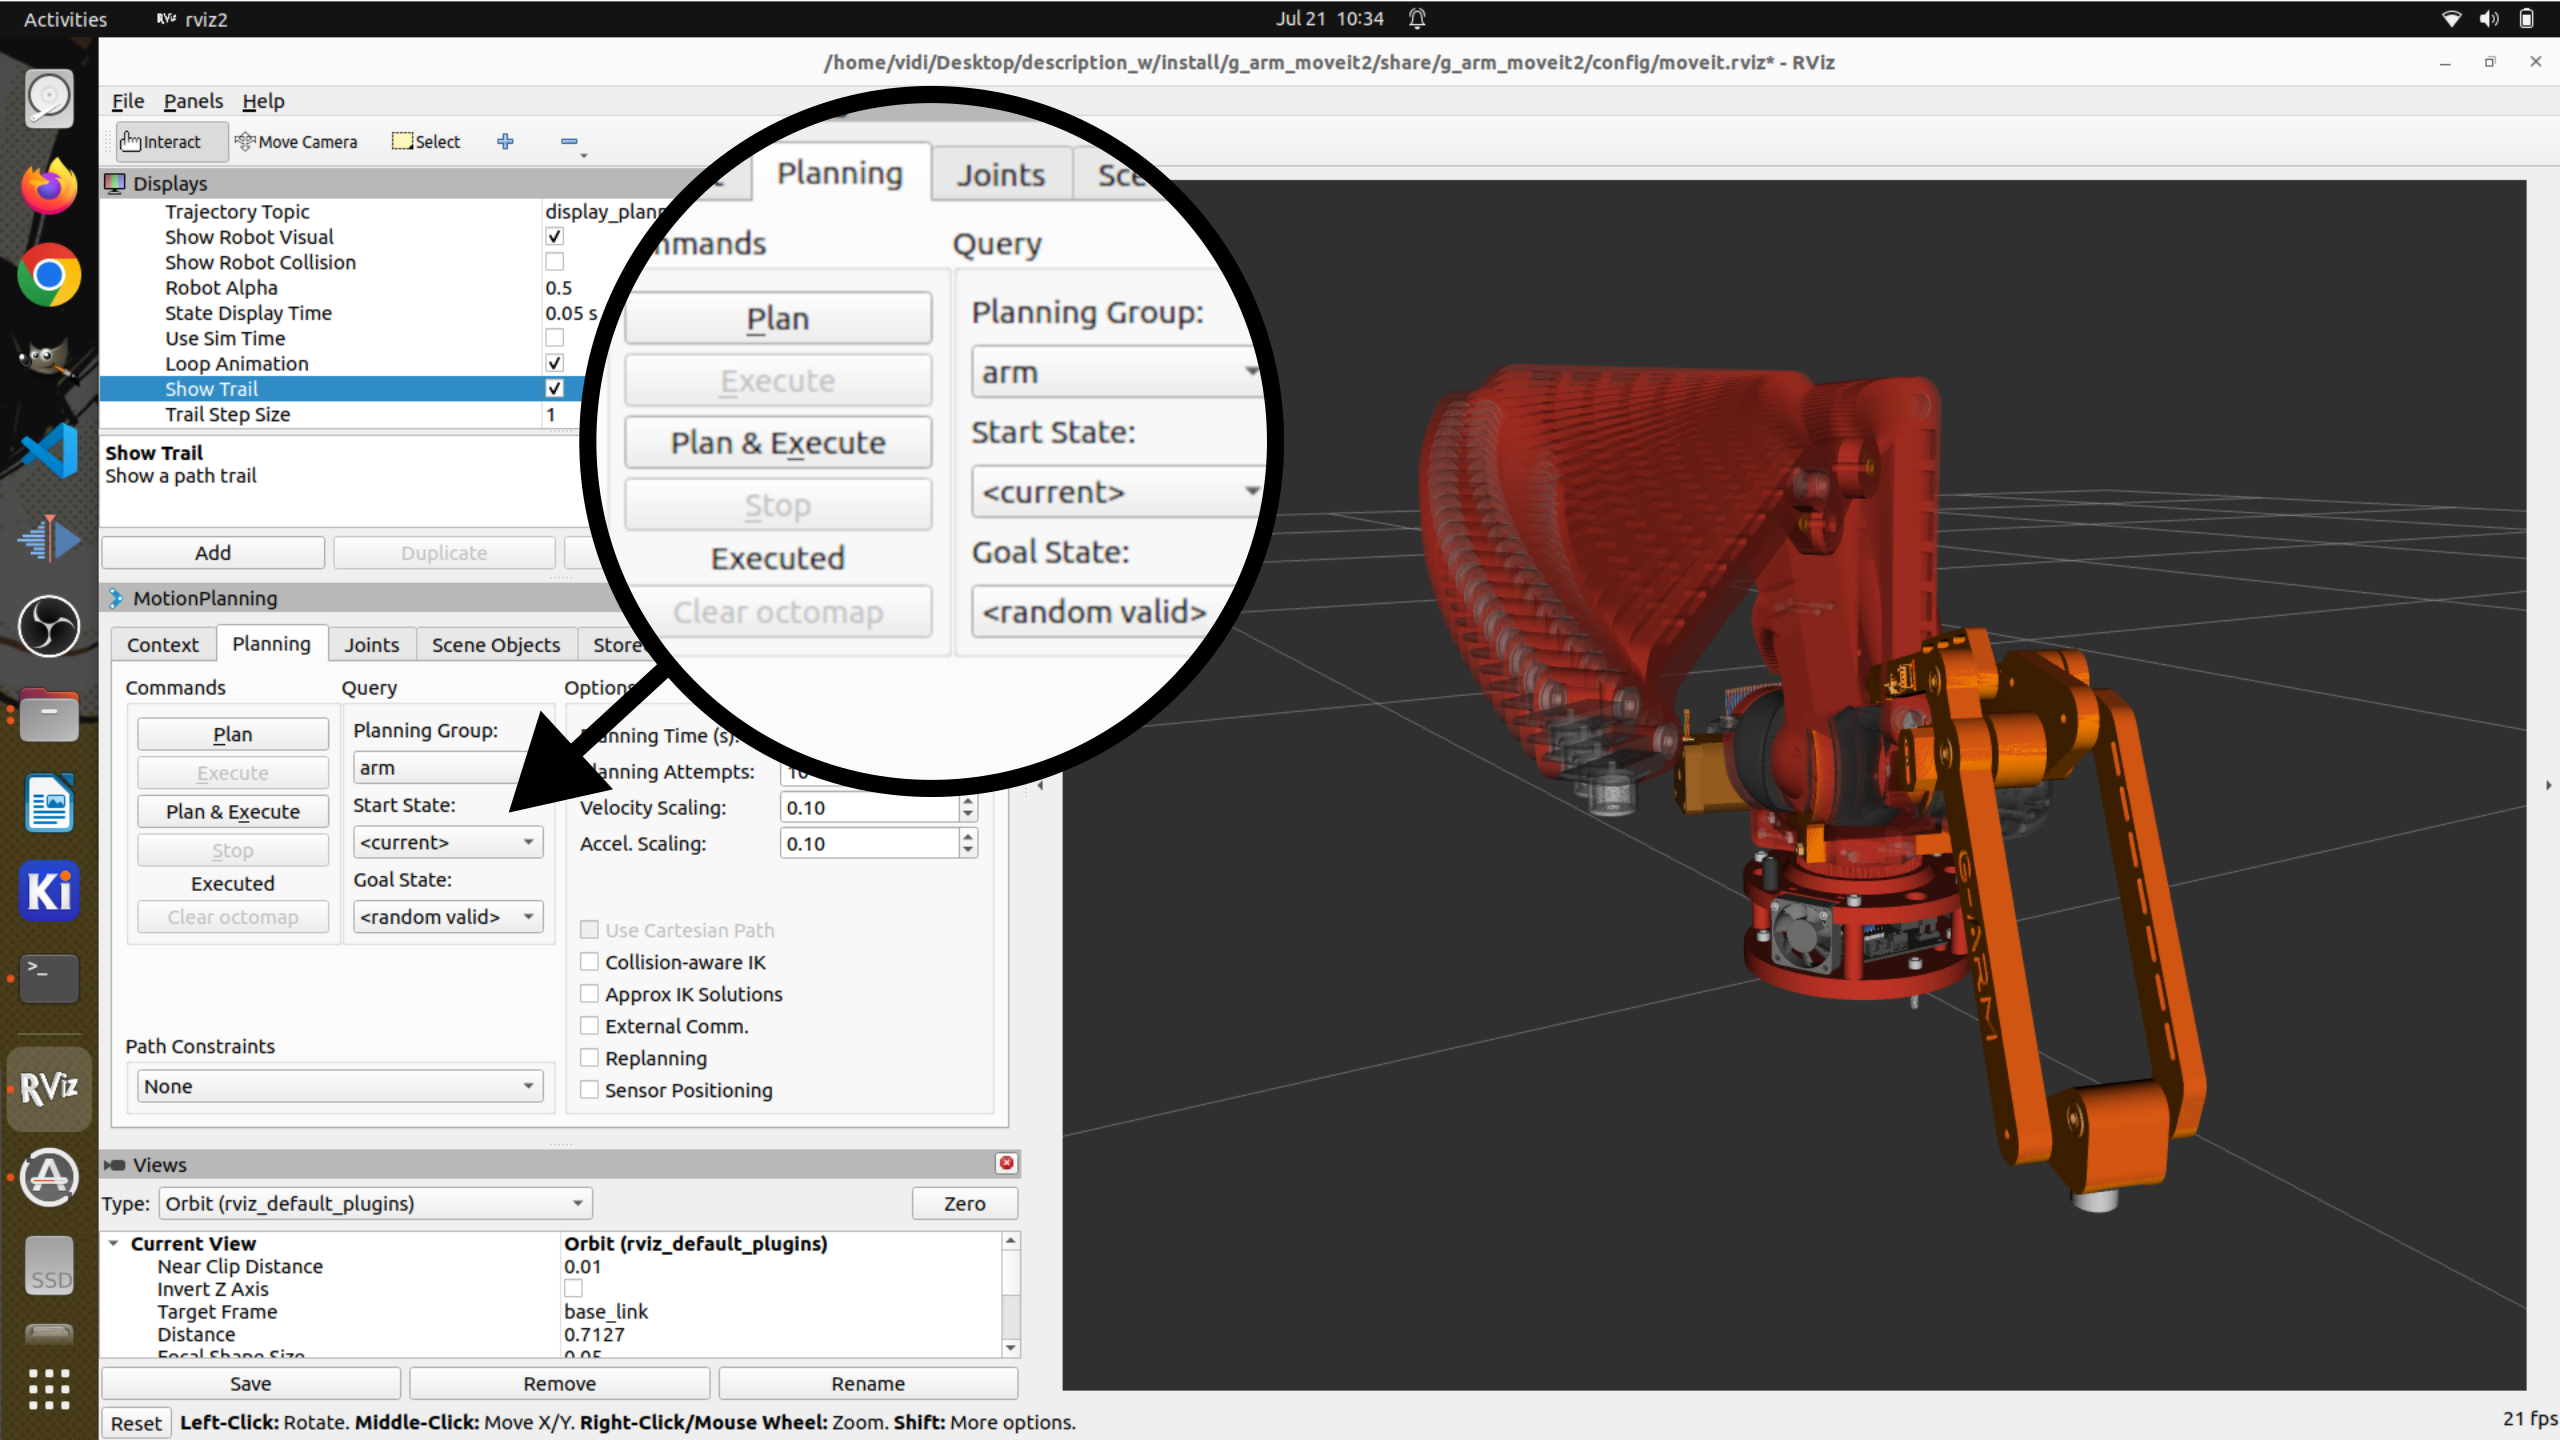
\includegraphics[width=0.65\textwidth, valign=m]{figs/moveit_demo_trajectory.png} 
  \end{tabular}
\end{table}  
\end{frame}

\begin{frame}
\frametitle{Arquitectura software}
    
\end{frame}

\section*{}
\begin{frame}{}
  \centering \Huge
  \emph{Pruebas técnicas}
\end{frame}

\section*{}
\begin{frame}{}
  \centering \Huge
  \emph{Conclusiones}
\note[item]{Para acabar esta presentación, vamos a repasar lo hecho, unas breves conclusiones y las líneas futuras.}
\end{frame}

\section{Conclusiones}
\begin{frame}
\begin{block}{Objetivos cumplidos}
\begin{itemize}
\item Herramienta multiplataforma: soporta Linux, Windows, MacOS.
\item Intuitiva para el usuario final: no se necesita instalar nada.
\item Solo se necesita un navegador web.
\end{itemize}
\end{block}

\begin{block}{Líneas futuras}
\begin{itemize}
\item Permitir el uso de otras herramientas.
\item Ampliar los botones disponibles en el interfaz.
\end{itemize}
\end{block}
\end{frame}

\begin{frame}[plain]
\large{\titlepage}
\note[item]{Y hasta aquí mi exposición.}
\note[item]{Quedo a disposición del tribunal...}
\end{frame}

\end{document}
